%% Beispiel-Präsentation
\documentclass[navbaroff,4:3]{kitbeamer} 

\usepackage{tikz}
\usetikzlibrary{automata}


\newcommand{\kit}[1]{\textcolor{kit-green100}{#1}}
\newcommand{\kitbf}[1]{\kit{\bf #1}}

%% Titelbild
\titleimage{key-wide}

%% Gruppenlogo
\grouplogo{} 

%% Gruppenname
\groupname{Institute of Theoretical Informatics}

% Beginn der Präsentation

\title{Specifying Components with Automata}
\subtitle{for the VerifyThis Long Term Challenge} 
\author{Mattias Ulbrich and Alexander Weigl}

\date[]{\today}

\begin{document}

%Titelseite
\KITtitleframe

\begin{frame}{Goal}

  \large

  \kitbf{It's about:} Show how an automaton specification can be used for Java
  component specification.

  \vfill

  \kitbf{It's \emph{not} about} inventing another automaton language.
  
\end{frame}

\begin{frame}{Hagrid as a component}

  [image from earlier presentation]

  \begin{itemize}
  \item operations receive and return immutable data
  \item operations modify a self-contained state 
  \item not every operation may be invoked at all times
  \end{itemize}
  
\end{frame}

%Inhaltsverzeichnis
\begin{frame}{Specifying Hagrid with an Automaton}

  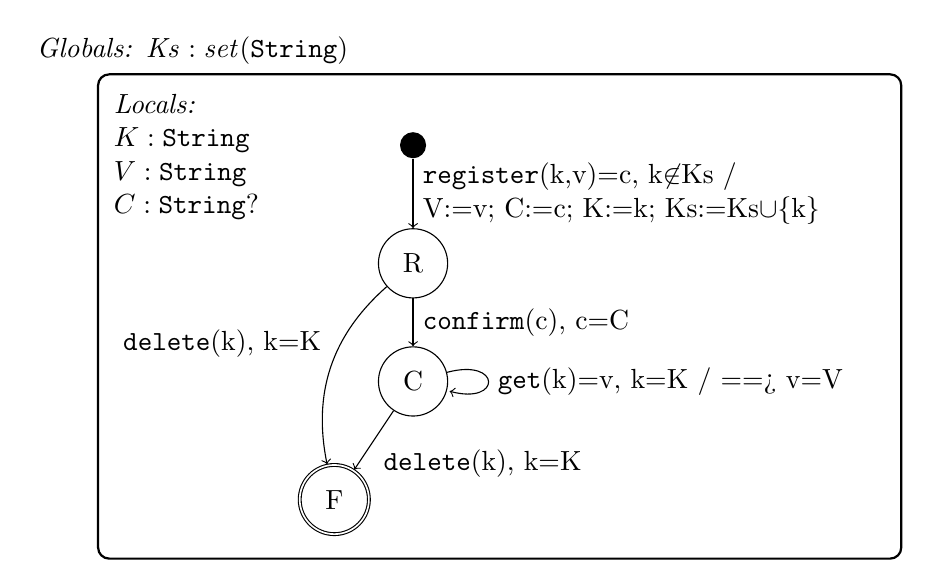
\begin{tikzpicture}[auto, ->, y=1.5cm]

      \draw[thick, rounded corners] (-3,-.5) rectangle (7.2, 3.6);
      
      \node[align=left] at (-1.8, 3.8) {\emph{Globals:} $\mathit{Ks} : \mathit{set}(\mathtt{String})$};
      
      \node[align=left, text width=2cm] at (-1.8, 2.9)
      {\emph{Locals:} \\
        $K: \mathtt{String}$ \\
        $V: \mathtt{String}$ \\
        $C: \mathtt{String}?$};
      
      \node[fill=black, circle] (empty) at (1, 3) {};
      \node[state] (registered) at (1, 2) {R};
      \node[state] (confirmed) at (1, 1) {C};
      \node[state, accepting] (finished) at (0,0) {F};
      
      \path
      (empty)      edge node[align=left, text width=6cm]
      {\texttt{register}(k,v)=c,  k$\not\in$Ks /\\
        V:=v; C:=c; K:=k; Ks:=Ks$\cup$\{k\}} (registered)
      (registered) edge node {\texttt{confirm}(c), c=C} (confirmed)
      (registered) edge[swap, bend right] node {\texttt{delete}(k), k=K} (finished)
      (confirmed)  edge node {\texttt{delete}(k), k=K} (finished)
      (confirmed)  edge[loop right] node {\texttt{get}(k)=v, k=K / ==> v=V} (confirmed);
    \end{tikzpicture}
  \end{frame}


\begin{frame}{Example state}

    \begin{tikzpicture}[auto, ->, y=1.5cm]
      \node[align=left] at (0, 3.8) {\emph{Globals:} $\mathit{Ks} = \kit{\{ a@x, b@x, c@x \}}$};
      
    \begin{scope}[xshift=-1cm]
      \draw[thick, rounded corners] (-1.2,-.5) rectangle (2.2, 3.6);
      
      \node[align=left, text width=2cm] at (-0., 2.9)
      {\emph{Locals:} \\
        $K = \kit{a@x}$ \\
        $V = \kit{KEY1}$ \\
        $C = \kit{CONF1}$};
      
      \node[fill=black, circle] (empty) at (1, 3) {};
      \node[state] (registered) at (1, 2) {R};
      \node[state, fill=kit-green50] (confirmed) at (1, 1) {C};
      \node[state, accepting] (finished) at (0,0) {F};
      
      \path
      (empty)      edge (registered)
      (registered) edge (confirmed)
      (registered) edge[bend right]  (finished)
      (confirmed)  edge (finished)
      (confirmed)  edge[loop right] (confirmed);
    \end{scope}
    \begin{scope}[xshift=3cm]
      \draw[thick, rounded corners] (-1.2,-.5) rectangle (2.2, 3.6);
      
      \node[align=left, text width=2cm] at (-0., 2.9)
      {\emph{Locals:} \\
        $K = \kit{b@x}$ \\
        $V = \kit{KEY2}$ \\
        $C = \kit{CONF2}$};
      
      \node[fill=black, circle] (empty) at (1, 3) {};
      \node[state] (registered) at (1, 2) {R};
      \node[state, fill=kit-green50] (confirmed) at (1, 1) {C};
      \node[state, accepting] (finished) at (0,0) {F};
      
      \path
      (empty)      edge (registered)
      (registered) edge (confirmed)
      (registered) edge[bend right]  (finished)
      (confirmed)  edge (finished)
      (confirmed)  edge[loop right] (confirmed);
    \end{scope}
    \begin{scope}[xshift=7cm]
      \draw[thick, rounded corners] (-1.2,-.5) rectangle (2.2, 3.6);
      
      \node[align=left, text width=2cm] at (-0., 2.9)
      {\emph{Locals:} \\
        $K = \kit{c@x}$ \\
        $V = \kit{KEY3}$ \\
        $C = \kit{CONF3}$};
      
      \node[fill=black, circle] (empty) at (1, 3) {};
      \node[state, fill=kit-green50] (registered) at (1, 2) {R};
      \node[state] (confirmed) at (1, 1) {C};
      \node[state, accepting] (finished) at (0,0) {F};
      
      \path
      (empty)      edge (registered)
      (registered) edge (confirmed)
      (registered) edge[bend right]  (finished)
      (confirmed)  edge (finished)
      (confirmed)  edge[loop right] (confirmed);
    \end{scope}

    \end{tikzpicture}
  
\end{frame}

\begin{frame}{Semantics}

  The automaton is a \textbf{stateful contract} for the component.

  \vfill
  
  It specifies
  \begin{itemize}
  \item which operations 
  \item with which parameters are allowed,
  \item and which operations are not allowed
  \end{itemize}
  depending on the current state.

  \begin{block}{Trace semantics}
    The semantics of a specification is the set of all traces of the
    automaton that satisfy all conditions.

    Trace: Sequence of parametrised operation invocations
  \end{block}
  
\end{frame}

\begin{frame}{The two faces of the interface}
  \begin{tikzpicture}

    \draw[thick, rounded corners, fill=kit-green15] (-5.6,3) rectangle (5.6,-3);
    \draw[thick, rounded corners, fill=kit-blue15] (0,2.5) rectangle (5.1,-2.5);

    \node[anchor=west] at (-5.6, 2.5) {\textbf{Outside:} Environment};
    \node[anchor=west] at (0, 2) {\textbf{Inside:} the component};

    \node[anchor=north west, text width=4cm] at (-5.6, 1.5) { \small
      \textbf{Obligations:}
      \begin{itemize}
      \item temporal properties
      \item protocol adherence (multi-component)
      \end{itemize}

      \textbf{Gains:}
      \begin{itemize}
      \item sound abstract from code
      \end{itemize}

      \textbf{Construct:} automata/proc algebra};

    \node[anchor=north west, text width=3cm] at (2, 1.5) { \small
      \textbf{Obligations:}
      \begin{itemize}
      \item contract conformance
      \end{itemize}

      \textbf{Gains:}
      \begin{itemize}
      \item temporal/protocol properties
      \end{itemize}

      \textbf{Construct:} contracts and ghost code};
  
   \node at (0,0) {\includegraphics[width=4cm]{automaton.png}};
  \end{tikzpicture}
\end{frame}

\end{document}
